\chapter{The Monte Carlo Random Walk Process for Radiation Transport}
\label{ch:particle_transport}
In the previous chapter, the Monte Carlo process was discussed in a very
general mathematical sense. In this chapter, it will be shown how to apply
the general Monte Carlo random walk process to radiation transport 
problems. This will require the derivation of the PDFs that govern the random 
walk process from the transport equation. This derivation will be done in
some detail so that each step of the derivation is very clear. The level of
detail will likely seem unnecessary because the PDFs that will be derived
will be very intuitive. However, PDFs for the dual problem, which will be
derived from the adjoint transport equation, will not be intuitive. 
Because the adjoint transport equation has a similar form to the
transport equation, the derivation will be similar. 

\section{The Integro-Differential Transport Equation}
\label{sec:int_diff_transport_eqn}
The equation that describes the average behavior of both charged and neutral
radiation in a medium is the transport equation. Several assumptions are made 
in the derivation of the transport equation, which is shown in equation 
\ref{eq:integro_diff_boltzmann_eqn} \citep{bell_nuclear_1979}. First, a neutral 
particle is assumed to be a point particle, which means that it can be 
completely characterized by its position and velocity. Second, the medium is 
assumed to contain a large enough number of neutral particles that deviations 
from the expected distribution of the particles can be ignored. In addition, 
the number of neutral particles present in the medium is not so large that they 
change the medium during the time scale of interest. Finally, particles 
are assumed to not interact with each other. This last assumption will be valid 
nearly always since even the highest density of particles that could potentially
be observed will still be significantly smaller than the density of the 
material in which the particles travel. The first assumption will not be valid 
for very low energy neutrons and for x-ray photons. However, if polarization 
and interference effects can be neglected, which will be the case in this 
report, this assumption is still acceptable. 
\begin{equation}
  \begin{split}
    \frac{1}{v}&\frac{\partial \varphi(\vec{r},E,\hat{\Omega},t)}{\partial t} +
    \hat{\Omega} \cdot \vec{\bigtriangledown} \varphi(\vec{r},E,\hat{\Omega},t)
    + \Sigma_T(\vec{r},E) \varphi(\vec{r},E,\hat{\Omega},t) = \\
    & \quad S(\vec{r},E,\hat{\Omega},t) +
    \int\int \Sigma_T(\vec{r},E^{'} \to E,\hat{\Omega^{'}} \to \hat{\Omega})
    \varphi(\vec{r},E^{'},\hat{\Omega^{'}},t) dE^{'}d\hat{\Omega^{'}} 
  \end{split}
  \label{eq:integro_diff_boltzmann_eqn}
\end{equation}
\begin{align}
  \vec{r} & = \text{spacial coordinate} \nonumber \\
  E & = \text{particle energy} \nonumber \\
  \hat{\Omega} & = \text{flight direction} \nonumber \\
  t & = \text{time} \nonumber \\
  v & = \text{particle speed} \nonumber \\
\end{align}

As mentioned previously, the transport equation only characterizes the average
or expected behavior of the radiation in a system. Therefore, the
continuous function, $\varphi(\vec{r},E,\hat{\Omega},t)$ in equation 
\ref{eq:integro_diff_boltzmann_eqn} can be interpreted as the expected particle 
flux at $\vec{r}$ and time $t$ for particles with energy $E$ and direction
$\hat{\Omega}$ per unit energy per unit solid angle. The external particle 
source density is described by the function $S(\vec{r},E,\hat{\Omega},t)$. It 
can be interpreted as the probability per unit time that a particle of energy 
$E$ will appear at $\vec{r}$ per unit volume per unit energy per unit solid 
angle. The function $\Sigma_T(\vec{r},E)$ describes the total macroscopic cross 
section at $\vec{r}$ for particles with energy $E$. It can be interpreted as the
probability of a particle interaction per unit distance of particle travel. In 
the context of photon transport it is often referred to as the attenuation 
coefficient. The doubly differential collision cross section is represented by 
the function $\Sigma_T(\vec{r},E^{'} \to E,\hat{\Omega}^{'} \to \hat{\Omega})$, 
which can be interpreted as the total probability per unit distance per unit 
energy per unit solid angle at $\vec{r}$ for the transfer of a particle with 
energy $E^{'}$ and direction $\hat{\Omega}^{'}$ to the energy $E$ and direction 
$\hat{\Omega}$ as a result of a collision. This doubly differential collision 
cross section can be expanded into a macroscopic cross section and a doubly 
differential transfer function. Also note that the total macroscopic cross 
section is just the sum of all partial macroscopic cross sections
\citep{bell_nuclear_1979}.
\begin{align}
  \Sigma_T(\vec{r},E^{'} \to E,\hat{\Omega}^{'} \to \hat{\Omega}) & =
  \Sigma_T(\vec{r},E^{'})
  f(\vec{r},E^{'} \to E,\hat{\Omega}^{'} \to \hat{\Omega}) \\
  & = \sum_i \Sigma_i(\vec{r},E^{'}) c_i(\vec{r},E^{'})
  f_i(\vec{r},E^{'} \to E,\hat{\Omega}^{'} \to \hat{\Omega})
  \label{eq:expanded_diff_collision_cross_sec}
\end{align}

Because the transport equation only takes into account average behavior, 
reactions that result in the emission of additional particles are handled 
implicitly. The doubly differential transfer probability can only describe the
average outgoing energy and direction distribution for all particles emitted
from the reaction. Some texts on neutron transport normalize the doubly
differential transfer probability for each reaction to the number of particles 
emitted from the reaction \citep{bell_nuclear_1979}. However, to facilitate 
sampling from these distributions, they will instead be normalized to unity. 
The number of particles emitted from reaction $i$ will then be accounted for by 
the function $c_i(\vec{r},E^{'})$. For absorption reactions like the 
(n,$\gamma$) and (n,$\alpha$) neutron reactions, the photoelectric effect for 
photons or the annihilation reaction for positrons, the function 
$c_i(\vec{r},E^{'})$ must be set equal to zero. For the elastic and inelastic 
scattering reactions of neutrons and gamma rays or the elastic scattering
reactions of electrons and positrons, the function $c_i(\vec{r},E^{'})$ will be 
set equal to unity. For the (n,2n) neutron reaction, the pair production photon 
reaction (neglecting charged particle creation) or the inelastic electron 
reaction, the function $c_i(\vec{r},E^{'})$ will be set equal to two. For 
fission reactions, the function $c_i(\vec{r},E^{'})$ will be set equal to the 
average number of neutrons produced by a fission caused by a neutron of energy 
$E^{'}$, $\nu(\vec{r},E^{'})$.

Based on these definitions for the function $c_i(\vec{r},E^{'})$ the 
normalization for the total transfer probability can be determined.
\begin{align}
  \int\int   \Sigma_T(\vec{r},E^{'})
  f(\vec{r},E^{'} \to E,\hat{\Omega}^{'} \to \hat{\Omega}) 
  dEd\hat{\Omega}
  & = \int\int \sum_i \Sigma_i(\vec{r},E^{'}) c_i(\vec{r},E^{'}) \nonumber \\
  & \qquad \quad \quad \cdot  
  f_i(\vec{r},E^{'} \to E,\hat{\Omega}^{'} \to \hat{\Omega}) 
  dEd\hat{\Omega} \nonumber \\
  \int\int f(\vec{r},E^{'} \to E,\hat{\Omega}^{'} \to \hat{\Omega}) 
  dEd\hat{\Omega} 
  & = \frac{\sum_i \Sigma_i(\vec{r},E^{'}) c_i(\vec{r},E^{'})}
             {\Sigma_T(\vec{r},E^{'})} \nonumber \\
  & = c(\vec{r},E^{'}) 
\end{align}
The function $c(\vec{r},E^{'})$ is the mean number of particles (of the same 
type as the primary) emerging per collision at $\vec{r}$ given a particle of 
energy $E^{'}$, which is a cross section weighted average of the 
$c_i(\vec{r},E^{'})$ functions.
  
While this consolidation of the transfer probabilities for each type of 
reaction into a single, average transfer function is necessary in the context 
of the transport equation, it is not necessary in a Monte Carlo random walk 
process. Instead, one can model each reaction type separately, use the 
detailed transfer probabilities for an associated reaction, and conduct 
a separate random walk for each additional particle emitted from a collision. 
Then, given a sufficient number of random walks, the behavior should be the 
same as if one were to use the averaged transfer function present in the 
transport equation\footnote{Generally, the creation of an average transfer
function that adequately described the behavior of the particle is quite
challenging. However, something close to this is often done in charged particle
transport due to the properties of the charged particle interaction cross
sections.}.

\section{The Transport equation in Integral Form}
The transport equation is often given in an integro-differential form, as seen 
in equation \ref{eq:integro_diff_boltzmann_eqn}. In order to use the Monte 
Carlo random walk process that was discussed in the previous chapter, the 
integro-differential form of the transport equation must be converted to a 
FIESK. Once it is in the appropriate form the PDFs that govern the random walk 
process for the radiation type of interest can be determined. Similar 
derivations to the one that will be shown can also be found in several 
references \citep{lewis_computational_1993, hoogenboom_adjoint_1977, irving_adjoint_1971, bell_nuclear_1979}.
 
In this report all problems discussed will be assumed to be steady state. 
Therefore, the time dependence of equation \ref{eq:integro_diff_boltzmann_eqn} 
will be ignored from here. To further simplify equation 
\ref{eq:integro_diff_boltzmann_eqn} the right hand side of the equation will be 
referred to simply as the emission density $\chi(\vec{r},E,\hat{\Omega})$.
\begin{equation}
    \chi(\vec{r},E,\hat{\Omega}) = S(\vec{r},E,\hat{\Omega}) +
    \int\int \Sigma_T(\vec{r},E^{'} \to E,\hat{\Omega}^{'} \to \hat{\Omega})
    \varphi(\vec{r},E^{'},\hat{\Omega}^{'}) dE^{'}d\hat{\Omega}^{'}
  \label{eq:emission_density}
\end{equation}
The reduced transport equation is shown in the following equation.
\begin{equation}
  \hat{\Omega} \cdot \vec{\bigtriangledown} \varphi(\vec{r},E,\hat{\Omega})
  + \Sigma_T(\vec{r},E) \varphi(\vec{r},E,\hat{\Omega}) =  
 \chi(\vec{r},E,\hat{\Omega})
  \label{eq:reduced_transport_eqn}
\end{equation}

From the reduced transport equation, the method of characteristics will be 
used to transform it to its integral form. The characteristic for the transport 
equation is the line defined by the fixed point $\vec{r}$ and the direction 
$\hat{\Omega}$. This line can be parameterized by the variable $R$ resulting in 
the following equation. 
\begin{equation}
  \vec{r}^{'} = \vec{r} - R\hat{\Omega}
  \label{eq:characteristic}
\end{equation}
Using equation \ref{eq:characteristic} a directional derivative along the
characteristic can be determined.
\begin{align}
  \frac{d}{dR} & = \frac{dx^{'}}{dR}\frac{\partial}{\partial x} +
  \frac{dy^{'}}{dR}\frac{\partial}{\partial y} +
  \frac{dz^{'}}{dR}\frac{\partial}{\partial z} \nonumber \\
  & = -\Omega_x \frac{\partial}{\partial x} -
  \Omega_y \frac{\partial}{\partial y} -
  \Omega_z \frac{\partial}{\partial z} \nonumber \\
  & = -\hat{\Omega} \cdot \vec{\bigtriangledown}
\end{align}
Using this directional derivative along the characteristic the transport 
equation can be reduced to a first order ordinary differential equation (ODE), 
which can be easily solved with the integrating factor
$exp\left[-\int_0^R \Sigma_T(\vec{r}-R^{'}\hat{\Omega},E)dR^{'} \right]$.
\begin{align}
  -\frac{d}{dR}\varphi(\vec{r}^{'},E,\hat{\Omega}) + \Sigma_T(\vec{r}^{'},E)
  \varphi(\vec{r}^{'},E,\hat{\Omega}) & =
  \chi(\vec{r}^{'},E,\hat{\Omega}) \nonumber \\
  -\frac{d}{dR}\bigg[\varphi(\vec{r}^{'},E,\hat{\Omega})
      exp\left[-\int_0^R \Sigma_T(\vec{r}-R^{'}\hat{\Omega},E)dR^{'}\right]
      \bigg] & = \nonumber \\
  \chi(\vec{r}^{'},E,\hat{\Omega})
  &exp\left[-\int_0^R \Sigma_T(\vec{r}-R^{'}\hat{\Omega},E)dR^{'} \right]
    \nonumber \\
    -\varphi(\vec{r} - R\hat{\Omega},E,\hat{\Omega})
    exp\left[-\int_0^R \Sigma_T(\vec{r}-R^{'}\hat{\Omega},E)dR^{'}\right] 
    \bigg|_0^{\infty} & = \nonumber \\
    \int_0^{\infty} 
    \chi(\vec{r} - R\hat{\Omega},E,\hat{\Omega})
    &exp\left[-\int_0^R \Sigma_T(\vec{r}-R^{'}\hat{\Omega},E)dR^{'} \right] dR
    \nonumber 
\end{align}
\begin{equation}
    \varphi(\vec{r},E,\hat{\Omega}) = 
    \int_0^{\infty} \chi(\vec{r} - R\hat{\Omega},E,\hat{\Omega})
    exp\left[-\int_0^R \Sigma_T(\vec{r}-R^{'}\hat{\Omega},E)dR^{'} \right] dR
  \label{eq:line_integral_transport_eqn}
\end{equation}
To get to equation \ref{eq:line_integral_transport_eqn} it was assumed that the
flux goes to zero as $R$ goes to infinity. This line integral will now be 
converted to an integral over all space. First, note that 
$R = |\vec{r} - \vec{r}^{'}|$, 
$\hat{\Omega} = \frac{\vec{r} - \vec{r}^{'}}{|\vec{r} - \vec{r}^{'}}|$ and
$dV^{'} = R^2dRd\hat{\Omega}$.
\begin{equation}
  \begin{split}
    \varphi(\vec{r},E,\hat{\Omega}) = 
    \int \chi(\vec{r}^{'},E,\hat{\Omega})
    exp\Big[-\int_0^{|\vec{r} - \vec{r}^{'}|} 
      &\Sigma_T(\vec{r}-R^{'}\hat{\Omega},E)dR^{'} \Big] \\
    &\cdot \frac{\delta \left(\Omega - \left[\frac{\vec{r} - \vec{r}^{'}}
        {|\vec{r} - \vec{r}^{'}|}\right]\right)}
    {|\vec{r} - \vec{r}^{'}|^2} dV^{'}
  \end{split}
  \label{eq:volume_integral_transport_eqn}
\end{equation}
With the transport equation now in an integral form, only minor manipulations
are needed in order to get it into a FIESK, after which point the random walk 
process can be determined.

\section{The Flux FIESK}
To get an equation that is only in terms of the flux, equation 
\ref{eq:emission_density} will be substituted back into equation 
\ref{eq:volume_integral_transport_eqn}.
\begin{equation*}
  \begin{split}
    \varphi(\vec{r},E,\hat{\Omega}) = \int &\left[
    S(\vec{r}^{'},E,\hat{\Omega}) + 
    \int\int \Sigma_T(\vec{r}^{'},E^{'} \to E, \hat{\Omega}^{'} \to \hat{\Omega})
    \varphi(\vec{r}^{'},E^{'},\hat{\Omega}^{'})dE^{'}d\hat{\Omega}^{'} \right] \\
    & \cdot exp\left[-\int_0^{|\vec{r} - \vec{r}^{'}|} 
      \Sigma_T(\vec{r}-R^{'}\hat{\Omega},E)dR^{'} \right]
    \cdot \frac{\delta \left(\Omega - \left[\frac{\vec{r} - \vec{r}^{'}}
        {|\vec{r} - \vec{r}^{'}|}\right]\right)} 
    {|\vec{r} - \vec{r}^{'}|^2} dV^{'}
  \end{split}
\end{equation*}

\begin{equation}
  \begin{split}
    \varphi(\vec{r},E,\hat{\Omega}) = & \int S(\vec{r}^{'},E,\hat{\Omega})
    \tau(\vec{r}^{'},\vec{r},E,\hat{\Omega}) dV^{'} + \\
    & \int\int\int \tau(\vec{r}^{'},\vec{r},E,\hat{\Omega})
    \Sigma_T(\vec{r}^{'},E^{'} \to E, \hat{\Omega}^{'} \to \hat{\Omega})
    \varphi(\vec{r}^{'},E^{'},\hat{\Omega}^{'}) dE^{'} d\hat{\Omega}^{'} dV^{'}
  \end{split}
  \label{eq:flux_integral_equation}
\end{equation}
The function $\tau(\vec{r}^{'},\vec{r},E,\hat{\Omega})$ is defined in the following 
equation.
\begin{equation}
  \tau(\vec{r}^{'},\vec{r},E,\hat{\Omega}) = 
  exp\left[-\int_0^{|\vec{r} - \vec{r}^{'}|} 
              \Sigma_T(\vec{r}-R^{'}\hat{\Omega},E)dR^{'} \right]
    \frac{\delta \left(\Omega - \left[\frac{\vec{r} - \vec{r}^{'}}
        {|\vec{r} - \vec{r}^{'}|}\right]\right)} 
    {|\vec{r} - \vec{r}^{'}|^2}
  \label{eq:unnormalized_transport_kernel}
\end{equation}

Equation \ref{eq:flux_integral_equation}, is a FIESK and a random walk process 
can therefore be created to simulate the flux. The source PDF will be created 
first. 
\begin{equation}
  p^1(\vec{r},E,\hat{\Omega}) = \frac{\int S(\vec{r}^{'},E,\hat{\Omega})
    \tau(\vec{r}^{'},\vec{r},E,\hat{\Omega}) dV^{'}}{\int\int S(\vec{r}^{'},E,\hat{\Omega})
    \tau(\vec{r}^{'},\vec{r},E,\hat{\Omega}) dV^{'} dV}
\end{equation}
The state transition PDF can be broken into two parts; one part will govern the
movement of the particle through space and the other part will govern the 
movement of the particle through energy and direction. Only the part that
governs the movement through space will be examined further.
\begin{equation}
  p(\vec{r}^{'} \to \vec{r}, E^{'} \to E, \hat{\Omega}^{'} \to \hat{\Omega}) =
  p(\vec{r}^{'} \to \vec{r}\quad| E,\hat{\Omega})
  p(E^{'} \to E, \hat{\Omega}^{'} \to \hat{\Omega}\quad|\vec{r}^{'})
\end{equation}
\begin{align}
  p(\vec{r}^{'} \to \vec{r} \quad | E,\hat{\Omega}) & =
  \frac{\tau(\vec{r}^{'},\vec{r},E,\hat{\Omega})}{w_1(\vec{r}^{'},E,\hat{\Omega})}  \\
  w_1(\vec{r}^{'},E,\hat{\Omega}) & = \int \tau(\vec{r}^{'},\vec{r},E,\hat{\Omega}) dV 
\end{align}

The random walk process that would correspond to the flux FIESK has many
disadvantages. First, during the random walk process, the weight of the 
particle after every collision will be multiplied by the factor $w_1$. 
Unfortunately, this factor is not bounded to the interval $(0,1)$ and will 
likely increase the variance of the estimator used. Another disadvantage of 
this random walk process comes about from the conditional state transition PDF 
$p(\vec{r}^{'} \to \vec{r}\quad| E,\hat{\Omega})$. Because this PDF does not 
contain the factor $\Sigma_T(\vec{r},E)$, it is possible to sample an event 
position in a vacuum. This peculiar property is due to the fact that the flux 
does not go to zero in a vacuum. The final disadvantage is that evaluating the 
source term would be challenging.

The Monte Carlo random walk process for estimating the flux directly is not 
ideal and in practice is rarely done. Clearly, an event density should have
a preferable random walk process because, intuitively, the event density
goes to zero in a vacuum. 

\section{The Emission Density FIESK}
A FIESK will now be constructed for the emission density. This is accomplished 
by substituting equation \ref{eq:volume_integral_transport_eqn}, which is the
integral form of the transport equation, into equation 
\ref{eq:emission_density}, which defines the emission density. 
\begin{align}
    \chi(\vec{r},E,\hat{\Omega}) & = S(\vec{r},E,\hat{\Omega}) +
    \int\int \Sigma_T(\vec{r},E^{'} \to E, \hat{\Omega}^{'} \to \hat{\Omega})
    \int \chi(\vec{r}^{'},E',\hat{\Omega}^{'}) \nonumber \\
    exp&\left[-\int_0^{|\vec{r} - \vec{r}^{'}|} 
      \Sigma_T(\vec{r}-R^{'}\hat{\Omega}^{'},E^{'})dR^{'} \right]
    \frac{\delta \left(\Omega^{'} - \left[\frac{\vec{r} - \vec{r}^{'}}
        {|\vec{r} - \vec{r}^{'}|}\right]\right)}
    {|\vec{r} - \vec{r}^{'}|^2} dV^{'}dE^{'}d\hat{\Omega}^{'} \nonumber \\
    \chi(\vec{r},E,\hat{\Omega}) & = S(\vec{r},E,\hat{\Omega}) + \nonumber \\
    & \qquad \quad
    \int_{\Gamma}C(\vec{r},E^{'} \to E,\hat{\Omega}^{'} \to \hat{\Omega})
    T(\vec{r}^{'} \to \vec{r},E^{'},\hat{\Omega}^{'}) 
    \chi(\vec{r}^{'},E',\hat{\Omega}^{'}) d\Gamma^{'}
  \label{eq:emission_density_integral_eqn}
\end{align}

The kernel $T(\vec{r}^{'} \to \vec{r},E,\hat{\Omega})$ is called the transport
kernel, which is defined in the next equation. The transport kernel is simply
the function $\tau(\vec{r}^{'},\vec{r},E,\hat{\Omega})$ defined in equation 
\ref{eq:unnormalized_transport_kernel} multiplied by the total cross section
$\Sigma_T(\vec{r},E)$. This causes the transport kernel to have the desirable
property that event locations cannot be sampled inside of a vacuum.
\begin{equation}
  \begin{split}
    T(\vec{r}^{'} \to \vec{r},&E,\hat{\Omega}) = \Sigma_T(\vec{r},E) \\
    &\cdot exp\left[-\int_0^{|\vec{r} - \vec{r}^{'}|} 
      \Sigma_T(\vec{r}-R^{'}\hat{\Omega},E)dR^{'} \right] 
    \frac{\delta \left(\Omega - \left[\frac{\vec{r} - \vec{r}^{'}}
        {|\vec{r} - \vec{r}^{'}|}\right]\right)}
    {|\vec{r} - \vec{r}^{'}|^2} 
  \end{split}
\end{equation}
The quantity $T(\vec{r}^{'} \to \vec{r},E,\hat{\Omega})dV$ can be interpreted
as the probability that a particle at $\vec{r}^{'}$ with energy $E$ and 
direction $\hat{\Omega}$ will have its next collision in volume element $dV$
at $\vec{r}$.  

The kernel $C(\vec{r},E^{'} \to E,\hat{\Omega}^{'} \to \hat{\Omega})$ is called
the collision kernel, which is defined in the next equation.
\begin{equation}
  C(\vec{r},E^{'} \to E,\hat{\Omega}^{'} \to \hat{\Omega}) = 
  \frac{\Sigma_T(\vec{r},E^{'} \to E,\hat{\Omega}^{'} \to \hat{\Omega})}
       {\Sigma_T(\vec{r},E^{'})}
\end{equation}

The transition and collision kernels can be combined to create a kernel that
characterizes the transition of a particle from a state 
$y = (\vec{r}^{'},E^{'},\hat{\Omega}^{'})$ of the phase space $\Gamma$ to another 
state $x = (\vec{r},E,\hat{\Omega})$. This new kernel is given in the following 
equation.
\begin{equation}
  K(y \to x) =
  C(\vec{r},E^{'} \to E,\hat{\Omega}^{'} \to \hat{\Omega})
    T(\vec{r}^{'} \to \vec{r},E^{'},\hat{\Omega}^{'})
\end{equation}
The integral equation of the emission density shown in equation 
\ref{eq:emission_density_integral_eqn} can now be represented as
\begin{equation*}
  \chi(x) = S(x) + \int_{\Gamma} K(y \to x)\chi(y)dy,
\end{equation*}
which is a FIESK. 

\section{The Collision Density FIESK}
Before taking a closer look at the kernel $K(y \to x)$, another quantity of 
interest must be discussed: the collision density. It is related to the
flux and the emission density by the following equations.
\begin{align}
  \psi(\vec{r},E,\hat{\Omega}) & = \Sigma_T(\vec{r},E)
  \varphi(\vec{r},E,\hat{\Omega}) \\
  & = \int T(\vec{r}^{'} \to \vec{r},E,\hat{\Omega})
  \chi(\vec{r}^{'},E,\hat{\Omega})dV^{'}
  \label{eq:collision_emission_relation}
\end{align}
Where as the emission density is the expected density of particles exiting a 
collision or the source, the collision density is the expected density of 
particles entering a collision. Using equation 
\ref{eq:collision_emission_relation} and equation \ref{eq:emission_density}, an 
integral equation for the collision density can be derived:
\begin{equation*}
  \psi(x) = S_c(x) + \int_{\Gamma} L(y \to x)\psi(y)dy.
\end{equation*}
In this equation $S_c(x)$ is the first collided source and $L(y \to x)$ is
a new kernel that also characterizes the transition of a particle from a state 
$y = (\vec{r}^{'},E^{'},\hat{\Omega}^{'})$ of the phase space $\Gamma$ to another 
state $x = (\vec{r},E,\hat{\Omega})$. These functions are defined in the 
following equations.
\begin{equation}
  S_c(x) = \int\int T(\vec{r}^{'} \to \vec{r},E,\hat{\Omega})
  S(\vec{r}^{'},E,\hat{\Omega})dV^{'}
\end{equation}
\begin{equation}
  L(y \to x) =
  T(\vec{r}^{'} \to \vec{r},E,\hat{\Omega})
  C(\vec{r'},E^{'} \to E,\hat{\Omega}^{'} \to \hat{\Omega})
\end{equation}

\section{Emission and Collision Density State Transition Kernel Properties}
Before the PDFs that govern the random walk process for the emission and
collision densities are derived, the transport and collision kernels must be 
investigated a bit further. First, note that for an infinite medium, the 
transport kernel is normalized. 
\begin{align}
  \int T(\vec{r}^{'} \to \vec{r},E,\hat{\Omega})dV & =
    \int \Sigma_T(\vec{r},E)
    \cdot exp\Big[-\int_0^{|\vec{r} - \vec{r}^{'}|} 
      \Sigma_T(\vec{r}-R^{'}\hat{\Omega},E)dR^{'} \Big] \nonumber \\
    & \qquad \qquad \qquad \qquad \qquad \qquad
    \frac{\delta \left(\Omega - \left[\frac{\vec{r} - \vec{r}^{'}}
        {|\vec{r} - \vec{r}^{'}|}\right]\right)}
    {|\vec{r} - \vec{r}^{'}|^2} dV \nonumber \\
  & = \int_0^{\infty} \Sigma_T(\vec{r}^{'}+R\hat{\Omega},E)
  \cdot exp\left[-\int_0^R \Sigma_T(\vec{r}^{'}+R^{''}\hat{\Omega},E)
    dR^{''} \right] dR \nonumber \\
  & = -\int_0^{\infty} \frac{d}{dR} exp\left[-\int_0^R 
    \Sigma_T(\vec{r}^{'}+R^{''}\hat{\Omega},E) dR^{''} \right] dR 
  \nonumber \\
  & = 1 \nonumber
\end{align}
However, if the domain of interest in a problem is finite, the transport kernel 
will no longer be normalized. Fortunately, this is taken care of by terminating 
random walks that exit the domain of interest, which is equivalent to 
surrounding the domain of interest with a purely absorbing medium of infinite 
extent \citep{irving_adjoint_1971}.

Based on equation \ref{eq:expanded_diff_collision_cross_sec}, the collision 
kernel is simply the total transfer probability.  
\begin{align}
  C(\vec{r},E^{'} \to E, \hat{\Omega}^{'} \to \hat{\Omega}) & =
  \frac{\Sigma_T(\vec{r},E^{'} \to E,\hat{\Omega}^{'} \to \hat{\Omega})}
       {\Sigma_T(\vec{r},E^{'})} \nonumber \\
  & = f(\vec{r},E^{'} \to E,\hat{\Omega}^{'} \to \hat{\Omega})
\end{align}
The collision kernel, being equal to the total transfer probability, has the 
following property. 
\begin{equation}
  \int\int C(\vec{r},E^{'} \to E,\hat{\Omega}^{'} \to \hat{\Omega}) 
  dEd\hat{\Omega} = c(\vec{r},E^{'})
  \label{eq:collision_op_prop_gen}
\end{equation}
In regions where either no multiplying reactions occur and/or the cross sections
for multiplying reactions are negligible, the collision kernel has the 
following, more familiar property.
\begin{align}
  \int\int C(\vec{r},E^{'} \to E,\hat{\Omega}^{'} \to \hat{\Omega}) 
  dEd\hat{\Omega} & = \frac{\Sigma_s(\vec{r},E^{'})}{\Sigma_T(\vec{r},E^{'})}
  \label{eq:collision_op_prop} \\
  & = P_{NA}(E^{'}) \nonumber 
\end{align}
The macroscopic cross section $\Sigma_s(\vec{r},E^{'})$ is the total macroscopic
scattering cross section. The ratio of the total macroscopic scattering cross
section and the total macroscopic cross section is often referred to as the 
non-absorption or survival probability, $P_{NA}(E)$. 

Based on properties of the transport and collision kernels, the properties of 
the emission density state transition kernel can be determined. The first
property, which is rather trivial, is that the emission density state 
transition kernel is always positive. The second property is that the 
normalization of the kernel is less than infinity. The kernel normalization, 
which is shown below, is $\bar{c}(\vec{r}^{'},E^{'})$. This function can be 
interpreted as an average of the mean number of particles emerging per 
collision along the line from $\vec{r}^{'}$ to $\vec{r}$ given a particle of 
energy $E^{'}$. Because there may be some regions of the system that are 
critical, the function $\bar{c}(\vec{r},E^{'})$ need not be less than one 
everywhere as long as the system as a whole is subcritical.
\begin{align}
  \int K(y \to x) dx & = \int\int\int 
  C(\vec{r},E^{'} \to E,\hat{\Omega}^{'} \to \hat{\Omega})
  T(\vec{r}^{'} \to \vec{r},E^{'},\hat{\Omega}^{'}) dE d\hat{\Omega} dV 
  \nonumber \\
  & = \int c(\vec{r},E^{'}) T(\vec{r}^{'} \to \vec{r},E^{'},\hat{\Omega}^{'})
  dV \nonumber \\
  & = \bar{c}(\vec{r}^{'},E^{'})
\end{align}

The properties of the collision density state transition kernel can also be
determined. Like the emission density state transition kernel, the collision
density state transition kernel is always positive. The kernel normalization, 
which is shown below, is $c(\vec{r},E^{'})$. This function is not strictly 
bounded to values less than one either since there may be regions of the system 
that are critical.
\begin{align}
  \int L(y \to x) dx & = \int\int\int
  T(\vec{r}^{'} \to \vec{r},E,\hat{\Omega})
  C(\vec{r}^{'},E^{'} \to E,\hat{\Omega}^{'} \to \hat{\Omega}) dV dE d\hat{\Omega}
  \nonumber \\
  & = \int\int 
  C(\vec{r}^{'},E^{'} \to E,\hat{\Omega}^{'} \to \hat{\Omega}) dE d\hat{\Omega} 
  \nonumber \\
  & = c(\vec{r}^{'},E^{'})
\end{align}

In the special case where only non-multiplying reactions occur in a system,
the function $c(\vec{r}^{'},E^{'})$ becomes the survival or non-absorption
probability $P_{NA}(\vec{r}^{'},E^{'})$, as explained before. The function
$\bar{c}(\vec{r}^{'},E^{'})$ becomes a spatial average of the non-absorption
probability, which will be referred to as $\overline{P}_{NA}(\vec{r}^{'},E^{'})$. 
The properties of the two state transition kernels are summarized below.
\begin{enumerate}
  \item $K(y \to x) > 0$ \\
    $L(y \to x) > 0$
  \item $\int K(y \to x)dx = \bar{c}(y) >= \overline{P}_{NA}(y)$ \\
    $\int L(y \to x)dx = c(y) >= P_{NA}(y)$
\end{enumerate}

Based on these properties for the two kernels, it would appear that 
conducting an analogue random walk process for radiation transport without 
using weights is impossible in a system where multiplying reactions are 
possible. This is indeed true if particle multiplication is handled implicitly. 
However, if particle multiplication is handled explicitly, with separate 
random walks conducted for each additional particle emitted, an analogue 
random walk process can be conducted without using weights. Handling
particle multiplication explicitly will require indirect sampling from the 
state transition kernels, which will be discussed in the next section.

\section{Indirect Sampling of the Collision Kernel}
As explained in the previous sections, sampling directly from the state
transition kernels is often not desirable (or even possible). In order to 
sample from the state transition kernels indirectly, the collision kernel 
must be expanded. 
\begin{align}
  C(\vec{r},E^{'} \to E, \hat{\Omega}^{'} \to \hat{\Omega}) & =
  \frac{\Sigma_T(\vec{r},E^{'} \to E,\hat{\Omega}^{'} \to \hat{\Omega})}
       {\Sigma_T(\vec{r},E^{'})} \nonumber \\
  & = f(\vec{r},E^{'} \to E,\hat{\Omega}^{'} \to \hat{\Omega}) \nonumber \\
  & = \sum_j \frac{\Sigma_j(\vec{r},E^{'})c_i(\vec{r},E^{'})
            f_i(\vec{r},E^{'} \to E,\hat{\Omega}^{'} \to \hat{\Omega})}
           {\Sigma_T(\vec{r},E^{'})} \nonumber \\
  & = \sum_A \frac{\Sigma_A(\vec{r},E^{'})}{\Sigma_T(\vec{r},E^{'})}
      \sum_j \frac{\sigma_{A,j}(E^{'})}{\sigma_A(E^{'})} c_{A,j}(E^{'})
      f_{A,j}(E^{'} \to E,\hat{\Omega}^{'} \to \hat{\Omega}) \nonumber \\
  & = \sum_A p_A(\vec{r},E^{'}) \sum_j p_{A,j}(E^{'}) 
      \sum_{k=1}^2 p_{A,j,k}(E^{'}) \nonumber \\
  & \qquad \qquad \qquad \qquad \qquad \quad
      \cdot \sum_{l=1}^{x_k} 
      f_{A,j,l}(E^{'} \to E,\hat{\Omega}^{'} \to \hat{\Omega})
  \label{eq:fully_expanded_collision_kernel}
\end{align}
In this expansion, the subscript $A$ denotes a particular nuclide or element, 
the subscript $j$ denotes a particular type of reaction and the subscript $l$ 
denotes a particular emitted particle. The function 
$f_{A,j,l}(E^{'} \to E,\hat{\Omega}^{'} \to \hat{\Omega})$ is the doubly
differential transfer probability for the initial particle and emitted
particle l given a collision of type j on nuclide or element A. This transfer 
probability will be normalized to unity. Since it is desired to conduct 
separate random walks for each emitted particle, only an integer number of 
particles can be emitted from a collision\footnote{The average number of 
particles emitted from fission will normally be a non-integer value}. The 
probabilities $p_{A,j,k}(E^{'})$ restrict the number of particles emitted to 
integer values. They are defined as follows along with the corresponding value 
of $x_k$.
\begin{align}
  p_{A,j,1} & =
  \begin{cases}
    \lceil c_{A,j}(E^{'}) \rceil - c_{A,j}(E^{'}) & \text{ if } c_{A,j}(E^{'})
    \text{ not an integer} \\
    1 & o.w.
  \end{cases} \\
  p_{A,j,2} & = 1 - p_{A,j,1}
\end{align}
\begin{align}
  x_1 & = 
  \begin{cases}
    \lfloor c_{A,j}(E^{'}) \rfloor & \text{ if } c_{A,j}(E^{'})
    \text{ not an integer} \\
    c_{A,j}(E^{'}) & o.w.
  \end{cases} \\
  x_2 & = \lceil c_{A,j}(E^{'}) \rceil
\end{align}
The expected value of the number of emitted particles, based on these probabilities and corresponding values of emitted particles, is $c_{A,j}(E^{'})$.

The process of indirectly sampling the collision kernel is now completely
defined by equation \ref{eq:fully_expanded_collision_kernel}. In this process,
one first samples the nuclide or element hit from the discrete PDF 
$p_A(\vec{r},E^{'})$. With the nuclide or element $A$ chosen, the reaction type 
is sampled from the discrete PDF $p_{A,j}(E^{'})$. The number of particles 
emitted from the collision, $x_k$, is then sampled from the discrete PDF 
$p_{A,j,k}(E^{'})$. Finally, for each emitted particle $l$, the outgoing energy 
and direction is sampled from the transfer probability 
$f_{A,j,l}(E^{'} \to E,\hat{\Omega}^{'} \to \hat{\Omega})$. In the sampling of the
reaction type, if an absorption reaction is chosen, the random walk for the 
current particle ends. Therefore, at every collision, a random walk will end 
with probability $\frac{\Sigma_A(\vec{r},E)}{\Sigma_T(\vec{r},E)}$. This 
behavior mimics the behavior that was described in the random walk process from 
the previous chapter. In addition, the particle weights will be unaffected by 
this sampling procedure.  

\section{The Emission and Collision Density Random Walk PDFs}
With the state transition kernels $K(y \to x)$ and $L(y \to x)$ fully 
characterized, the Monte Carlo random walk process for radiation can 
be completely specified. The first set of processes is for treating 
multiplication implicitly\footnote{It must be noted that the random walk 
procedures that treat multiplication implicitly will never be used. This is 
because they rely on the total transfer probability, which is challenging to 
obtain and even more challenging to sample from directly. However, they are 
shown to provide continuity between this chapter and the previous chapter.}. 
The second set is for treating multiplication explicitly using the procedure 
outlined in the previous section. In the second set of processes, the 
termination probabilities aren't sampled directly. Instead, a random walk can 
potentially be terminated when sampling from $p(y \to x)$.
\begin{align}
  \chi(x)\text{ Random Walk (implicit mult.):}&
  \begin{cases}
    p^1(x) & = \frac{S(x)}{\int_{\Gamma} S(x)dx} \\
    p(y \to x) &  = \frac{\overline{P}_{NA}(y)}{\bar{c}(y)}K(y \to x) \\
    p(x) & = 1 - \overline{P}_{NA}(x)
  \end{cases} \\
  \psi(x)\text{ Random Walk (implicit mult.):}&
  \begin{cases}
    p^1(x) & = \frac{S_c(x)}{\int_{\Gamma} S_c(x)dx} \\
    p(y \to x) & = \frac{P_{NA}(y)}{c(y)}L(y \to x) \\
    p(x) & = 1 - P_{NA}(x)
  \end{cases} \\
  \nonumber \\
  \chi(x)\text{ Random Walk (explicit mult.):} &
  \begin{cases}
    p^1(x) & = \frac{S(x)}{\int_{\Gamma} S(x)dx} \\
    p(y \to x) &  = K(y \to x) \\
    p(x) & = 1 - \overline{P}_{NA}(x)
  \end{cases}
  \label{eq:mc_random_walk_emission_dens} \\
  \psi(x)\text{ Random Walk (explicit mult.):} &
  \begin{cases}
    p^1(x) & = \frac{S_c(x)}{\int_{\Gamma} S_c(x)dx} \\
    p(y \to x) & = L(y \to x) \\
    p(x) & = 1 - P_{NA}(x)
  \end{cases}
  \label{eq:mc_random_walk_collision_dens}
\end{align}

While it might appear from the above PDFs that the random walk processes for
the emission and collision density are completely different, because the kernels
$K(y \to x)$ and $L(y \to x)$ only differ in the ordering of the collision and 
transport kernels and because of the relationship between the emission density 
and the collision density, both of these quantities can be estimated during the 
same random walk process. Figure \ref{fig:combined_random_walk_process} 
illustrates the new combined random walk process. In this new process, 
particles always start in the true source and not the first collided source, 
which is advantageous because the first collided source would be challenging to 
calculate. The emission density will always be estimated right after a collision
(or birth) and the collision density will always be estimated right before a 
collision. This combined process will also prove advantageous when using either 
of the estimators that were described in the previous chapter. The next section 
will elaborate on this point.
\begin{figure}[t!]
  \begin{center}
    \scalebox{0.75}{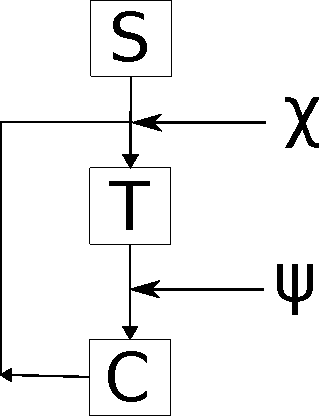
\includegraphics{chapters/random_walk_process_derivation/random_walk_process.pdf}}
    \end{center}
  \caption{\textbf{Monte Carlo random walk procedure for radiation.}
    \textit{A particle state is first sampled from the source distribution. The
      next collision point is sampled from the transport kernel T. Finally,
      the new particle energy and direction is sampled from the collision
      kernel, assuming that an absorption reaction wasn't sampled. If an
      absorption reaction was sampled, the random walk ends. Otherwise, the
      process continues. This procedure allows both the emission density and 
      the collision density to be estimated.}}
  \label{fig:combined_random_walk_process}
\end{figure}

A common modification to the previous analogue random walk processes is to 
ignore absorption. This modification results in the following non-analogue
random walk processes. 
\begin{align}
  \chi(x)\text{ Random Walk (implicit mult.):}&
  \begin{cases}
    p^1(x) & = \frac{S(x)}{\int_{\Gamma} S(x)dx} \\
    p(y \to x) &  = \frac{K(y \to x)}{\bar{c}(y)} \\
    p(x) & = 0
  \end{cases} \\
  \psi(x)\text{ Random Walk (implicit mult.):}&
  \begin{cases}
    p^1(x) & = \frac{S_c(x)}{\int_{\Gamma} S_c(x)dx} \\
    p(y \to x) & = \frac{L(y \to x) }{c(y)} \\
    p(x) & = 0
  \end{cases} \\
  \nonumber \\
  \chi(x)\text{ Random Walk (explicit mult.):}&
  \begin{cases}
    p^1(x) & = \frac{S(x)}{\int_{\Gamma} S(x)dx} \\
    p(y \to x) &  = \frac{K(y \to x)}{\overline{P}_{NA}(x)} \\
    p(x) & = 0
  \end{cases}
  \label{eq:mc_random_walk_emission_dens_nonan} \\
  \psi(x)\text{ Random Walk (explicit mult.):} &
  \begin{cases}
    p^1(x) & = \frac{\psi_1(x)}{\int_{\Gamma}\psi_1(x)dx} \\
    p(y \to x) & = \frac{L(y \to x)}{P_{NA}(x)} \\
    p(x) & = 0
  \end{cases}
  \label{eq:mc_random_walk_collision_dens_nonan}
\end{align}
Russian roulette will have to be used with these random walk processes to 
force random walks to terminate when the particle weight becomes too small. 

\section{Estimating Responses}
In typical radiation transport problems, the inner product of some 
function $a(\vec{r},E,\hat{\Omega})$ and the flux 
$\varphi(\vec{r},E,\hat{\Omega})$ is desired. If the function 
$a(\vec{r},E,\hat{\Omega})$ is a cross section, the inner product that is 
calculated is often called a material response or reaction rate. Because it is 
challenging to estimate the flux directly using a Monte Carlo random walk 
procedure, equivalent inner products must be constructed that are either in 
terms of the collision density or the emission density. 
\begin{align}
  I & = \int a(\vec{r},E,\hat{\Omega}) \varphi(\vec{r},E,\hat{\Omega}) 
  dVdEd\hat{\Omega} \\
  & = \int b(\vec{r},E,\hat{\Omega}) \psi(\vec{r},E,\hat{\Omega})  
  dVdEd\hat{\Omega} \\
  & = \int c(\vec{r},E,\hat{\Omega}) \chi(\vec{r},E,\hat{\Omega}) 
  dVdEd\hat{\Omega}
\end{align}
Based on the relationship between the collision density and the flux, $b(x)$
must be defined as follows, where $\Sigma_T(x)$ is the total cross section.
\begin{equation}
  b(\vec{r},E,\hat{\Omega}) = \frac{a(\vec{r},E,\hat{\Omega})}
  {\Sigma_T(\vec{r},E)}
  \label{eq:collision_response_function}
\end{equation}
Similarly, the function $c(x)$ must be defined as follows.
\begin{equation}
  c(\vec{r},E,\hat{\Omega}) = \int \frac{a(\vec{r}^{'},E,\hat{\Omega})}
  {\Sigma_T(\vec{r}^{'},E)} T(\vec{r} \to \vec{r}^{'},E,\Omega)dV'
  \label{eq:emission_response_function}
\end{equation}

Clearly, the function $b(\vec{r},E,\hat{\Omega})$ will be easier to evaluate, 
which presents an interesting trade-off. Estimators will be easier to use if 
the random walk process for the collision density is used. However, the random 
walk process for the collision density will be harder to conduct than the 
random walk process for the emission density because of the difficulty in 
evaluating the first collided source. Fortunately, the combined random walk 
process allows one to take advantage of the function 
$b(\vec{r},E,\hat{\Omega})$ without ever having to evaluate the first collided 
source. 

In chapter \ref{ch:mc_methods}, two very general estimators were introduced.
When one is dealing with the transport equation, there is another estimator 
called the track length estimator that can be used. A derivation of this 
estimator, which is a limiting case of the event estimator, can be found in ref.
\citep{spanier_monte_1969}. If the function $a(\vec{r},E,\hat{\Omega})$ is 
assumed to have the following form, then the track length estimator can be 
defined. 
\begin{equation*}
  a(\vec{r},E,\hat{\Omega}) = 
  \begin{cases}
    f(\vec{r},E,\hat{\Omega}) & \text{ if } \vec{r} \in V_d \\
    0 & \text{ o.w.}
  \end{cases}
\end{equation*}

\begin{equation}
  \eta^{*}(\alpha) = \sum_m W_m(\alpha)f_md_m
\end{equation}
The value $d_m$ is simply the length of the $m^{th}$ particle track in the 
volume $V_d$. The value $f_m$ is the value of the function 
$f(\vec{r},E,\hat{\Omega})$ along the $m^{th}$ particle track. 
